%include part: see main.beamer.tex and main.article.tex
%include common packages and settings
\usepackage{etex} %эта магическая херь избавляет от переполнения регистров TeX а!!!

\mode<article>{\usepackage{fullpage}}
\mode<presentation>{
    \usetheme{Madrid} %%Boadilla,Madrid,AnnArbor,CambridgeUS,Malmoe,Singapore,Berlin
    \useoutertheme{shadow}
} 

\usepackage[utf8]{inputenc}
\usepackage[russian]{babel}
\usepackage{indentfirst}
\usepackage{graphicx}

\usepackage{amsmath}
\usepackage{amsfonts}
\usepackage{amsthm}
\usepackage{algorithm}
\usepackage{algorithmic}

\usepackage[all]{xy}

\date{Лекция по дисциплине <<информатика>>\\(\today)}
\author[М.~М.~Шихов]{Михаил Шихов \\ \texttt{\underline{m.m.shihov@gmail.com}}}

%для рисования графов пакетом xy-pic
\entrymodifiers={++[o][F-]}

%для псевдокода алгоритмов (algorithm,algorithmic)
\renewcommand{\algorithmicrequire}{\textbf{Вход:}}
\renewcommand{\algorithmicensure}{\textbf{Выход:}}
\renewcommand{\algorithmiccomment}[1]{// #1}
\floatname{algorithm}{Псевдокод}

%%определённые мной команды логической разметки
\newcommand{\DC}[1]{\text{ДК}(#1)}
\newcommand{\MDC}[1]{\text{MДК}(#1)}
\newcommand{\OC}[1]{\text{ОК}(#1)}
\newcommand{\MOC}[1]{\text{МОК}(#1)}
\newcommand{\PC}[1]{\text{ПК}(#1)}

\newcommand{\Machine}[1]{\texttt{#1}}

\newcommand{\UnsignedAny}[2]{\text{\upshape
    \begin{tabular}{lr}
        \tiny{#1} & \tiny{0}\\ 
        \hline
        \multicolumn{2}{|c|}{\Machine{#2}} \\ 
        \hline
    \end{tabular}
}}

\newcommand{\UnsignedByte}[1]{\UnsignedAny{7}{#1}}

\newcommand{\UnsignedTwoBytes}[1]{\UnsignedAny{15}{#1}}

\newcommand{\SignedAny}[4]{\text{\upshape
    \begin{tabular}{clr}
        \tiny{#1}  &\tiny{#2} & \tiny{0}\\ 
        \hline
        \multicolumn{1}{|c|}{\Machine{#3}} & \multicolumn{2}{|c|}{\Machine{#4}} \\ 
        \hline
    \end{tabular}
}}

\newcommand{\SignedNibble}[2]{\SignedAny{3}{2}{#1}{#2}}

\newcommand{\SignedByte}[2]{\SignedAny{7}{6}{#1}{#2}}

\newcommand{\SignedTwoBytes}[2]{\SignedAny{15}{14}{#1}{#2}}

\newcommand{\FloatMyHex}[4]{\text{\upshape
    \begin{tabular}{clrclr}
        \tiny{15}  &\tiny{14} & \tiny{6} & \tiny{5} & \tiny{4} & \tiny{0}\\ 
        \hline
        \multicolumn{1}{|c|}{\texttt{#1}} 
            & \multicolumn{2}{|c|}{\texttt{#2}} 
                & \multicolumn{1}{|c|}{\texttt{#3}} 
                    & \multicolumn{2}{|c|}{\texttt{#4}} \\ 
        \hline
    \end{tabular}
}}

\newcommand{\FloatMyCharHex}[3]{\text{\upshape
    \begin{tabular}{clrlr}
        \tiny{15}  &\tiny{14} & \tiny{6} & \tiny{5} & \tiny{0}\\ 
        \hline
        \multicolumn{1}{|c|}{\texttt{#1}} 
            & \multicolumn{2}{|c|}{\texttt{#2}} 
                & \multicolumn{2}{|c|}{\texttt{#3}} \\ 
        \hline
    \end{tabular}
}}

\newcommand{\FloatMySimpleHex}[2]{\text{\upshape
    \begin{tabular}{lrlr}
        \tiny{15}  & \tiny{6} & \tiny{5} & \tiny{0} \\ 
        \hline
        \multicolumn{2}{|c|}{\texttt{#1}} 
            & \multicolumn{2}{|c|}{\texttt{#2}} \\ 
        \hline
    \end{tabular}
}}

\newcommand{\FloatMyOrderX}[4]{\text{\upshape
    \begin{tabular}{clrclr}
        \tiny{9}  &\tiny{8} & \tiny{4} & \tiny{3} & \tiny{2} & \tiny{0}\\ 
        \hline
        \multicolumn{1}{|c|}{\texttt{#1}} 
            & \multicolumn{2}{|c|}{\texttt{#2}} 
                & \multicolumn{1}{|c|}{\texttt{#3}} 
                    & \multicolumn{2}{|c|}{\texttt{#4}} \\ 
        \hline
    \end{tabular}
}}

\newcommand{\FloatMyDcOrderX}[3]{\text{\upshape
    \begin{tabular}{lrclr}
        \tiny{9} & \tiny{4} & \tiny{3} & \tiny{2} & \tiny{0}\\ 
        \hline
        \multicolumn{2}{|c|}{\texttt{#1}} 
            & \multicolumn{1}{|c|}{\texttt{#2}} 
                & \multicolumn{2}{|c|}{\texttt{#3}} \\ 
        \hline
    \end{tabular}
}}

\newcommand{\FloatMyDcCharX}[2]{\text{\upshape
    \begin{tabular}{lrlr}
        \tiny{9} & \tiny{4} & \tiny{3} & \tiny{0}\\ 
        \hline
        \multicolumn{2}{|c|}{\texttt{#1}} 
            & \multicolumn{2}{|c|}{\texttt{#2}} \\ 
        \hline
    \end{tabular}
}}

\newcommand{\FloatMyCharX}[3]{\text{\upshape
    \begin{tabular}{clrlr}
        \tiny{9}  &\tiny{8} & \tiny{4} & \tiny{3} & \tiny{0}\\ 
        \hline
        \multicolumn{1}{|c|}{\texttt{#1}} 
            & \multicolumn{2}{|c|}{\texttt{#2}} 
                & \multicolumn{2}{|c|}{\texttt{#3}} \\ 
        \hline
    \end{tabular}
}}

\newcommand{\FloatESShort}[3]{\text{\upshape
    \begin{tabular}{clrlr}
        \tiny{31}  &\tiny{30} & \tiny{24} & \tiny{23} & \tiny{0}\\ 
        \hline
        \multicolumn{1}{|c|}{\texttt{#1}} 
            & \multicolumn{2}{|c|}{\texttt{#2}} 
                & \multicolumn{2}{|c|}{\texttt{#3}} 
                    \\ 
        \hline
    \end{tabular}
}}

\newcommand{\FloatPCShort}[3]{\text{\upshape
    \begin{tabular}{clrlr}
        \tiny{31}  &\tiny{30} & \tiny{23} & \tiny{22} & \tiny{0}\\ 
        \hline
        \multicolumn{1}{|c|}{\texttt{#1}} 
            & \multicolumn{2}{|c|}{\texttt{#2}} 
                & \multicolumn{2}{|c|}{\texttt{#3}} 
                    \\ 
        \hline
    \end{tabular}
}}


%--- СПЕЦИФИЧНЫЕ ДЛЯ УМНОЖЕНИЯ КОМАНДЫ ---------------------------------------------------------------------------------------------


\newcommand{\Number}[1]{
    \texttt{#1}
}

\newcommand{\NumberHi}[2]{
    \underline{\underline{\texttt{#1}}}\texttt{#2}
}

\newcommand{\NumberMid}[3]{
    \texttt{#1}\underline{\underline{\texttt{#2}}}\texttt{#3}
}

\newcommand{\NumberLo}[2]{
    \texttt{#1}\underline{\underline{\texttt{#2}}}
}

\newcommand{\Stack}[2]{
    \begin{tabular}[t]{@{}r@{}}
        {#1}\\ \hline
        {#2}\\ 
    \end{tabular}
}

\newcommand{\Operation}[4]{
    \begin{tabular}[t]{@{}r@{}}
        \texttt{#4}
        \begin{tabular}{@{}r@{}}
            \Number{#1}\\
            \Number{#2}\\ \hline
        \end{tabular} \\ 
        \Number{#3}\\
    \end{tabular}
}

\newcommand{\Addition}[3]{\Operation{#1}{#2}{#3}{+}}

\newcommand{\Subtraction}[3]{\Operation{#1}{#2}{#3}{-}}

\newcommand{\Multiplication}[3]{\Operation{#1}{#2}{#3}{$\times$}}

\newcommand{\Register}[2]{\Number{#1:#2}}

\newcommand{\Mantiss}{m}
\newcommand{\Order}{p}
\newcommand{\Char}{c}

\newcommand{\MantissOf}[1]{\Mantiss_{#1}}
\newcommand{\OrderOf}[1]{\Order_{#1}}
\newcommand{\CharOf}[1]{\Char_{#1}}

\newcommand{\FloatExpression}[2]{\MantissOf{#1}\cdot {#2}^{\OrderOf{#1}}}

\newenvironment{Solve}[1]%
    {\begin{proof}[Решение]#1}
    {\end{proof}}
    
    
%определённые мной команды логической разметки
\newcommand{\DC}[1]{\text{ДК}(#1)}
\newcommand{\MDC}[1]{\text{MДК}(#1)}
\newcommand{\OC}[1]{\text{ОК}(#1)}
\newcommand{\MOC}[1]{\text{МОК}(#1)}
\newcommand{\PC}[1]{\text{ПК}(#1)}

\newcommand{\Machine}[1]{\texttt{#1}}

\newcommand{\UnsignedAny}[2]{\text{\upshape
    \begin{tabular}{lr}
        \tiny{#1} & \tiny{0}\\ 
        \hline
        \multicolumn{2}{|c|}{\Machine{#2}} \\ 
        \hline
    \end{tabular}
}}

\newcommand{\UnsignedByte}[1]{\UnsignedAny{7}{#1}}

\newcommand{\UnsignedTwoBytes}[1]{\UnsignedAny{15}{#1}}

\newcommand{\SignedAny}[4]{\text{\upshape
    \begin{tabular}{clr}
        \tiny{#1}  &\tiny{#2} & \tiny{0}\\ 
        \hline
        \multicolumn{1}{|c|}{\Machine{#3}} & \multicolumn{2}{|c|}{\Machine{#4}} \\ 
        \hline
    \end{tabular}
}}

\newcommand{\SignedNibble}[2]{\SignedAny{3}{2}{#1}{#2}}

\newcommand{\SignedByte}[2]{\SignedAny{7}{6}{#1}{#2}}

\newcommand{\SignedTwoBytes}[2]{\SignedAny{15}{14}{#1}{#2}}

\newcommand{\FloatMyHex}[4]{\text{\upshape
    \begin{tabular}{clrclr}
        \tiny{15}  &\tiny{14} & \tiny{6} & \tiny{5} & \tiny{4} & \tiny{0}\\ 
        \hline
        \multicolumn{1}{|c|}{\texttt{#1}} 
            & \multicolumn{2}{|c|}{\texttt{#2}} 
                & \multicolumn{1}{|c|}{\texttt{#3}} 
                    & \multicolumn{2}{|c|}{\texttt{#4}} \\ 
        \hline
    \end{tabular}
}}

\newcommand{\FloatMyCharHex}[3]{\text{\upshape
    \begin{tabular}{clrlr}
        \tiny{15}  &\tiny{14} & \tiny{6} & \tiny{5} & \tiny{0}\\ 
        \hline
        \multicolumn{1}{|c|}{\texttt{#1}} 
            & \multicolumn{2}{|c|}{\texttt{#2}} 
                & \multicolumn{2}{|c|}{\texttt{#3}} \\ 
        \hline
    \end{tabular}
}}

\newcommand{\FloatMySimpleHex}[2]{\text{\upshape
    \begin{tabular}{lrlr}
        \tiny{15}  & \tiny{6} & \tiny{5} & \tiny{0} \\ 
        \hline
        \multicolumn{2}{|c|}{\texttt{#1}} 
            & \multicolumn{2}{|c|}{\texttt{#2}} \\ 
        \hline
    \end{tabular}
}}

\newcommand{\FloatMyOrderX}[4]{\text{\upshape
    \begin{tabular}{clrclr}
        \tiny{9}  &\tiny{8} & \tiny{4} & \tiny{3} & \tiny{2} & \tiny{0}\\ 
        \hline
        \multicolumn{1}{|c|}{\texttt{#1}} 
            & \multicolumn{2}{|c|}{\texttt{#2}} 
                & \multicolumn{1}{|c|}{\texttt{#3}} 
                    & \multicolumn{2}{|c|}{\texttt{#4}} \\ 
        \hline
    \end{tabular}
}}

\newcommand{\FloatMyDcOrderX}[3]{\text{\upshape
    \begin{tabular}{lrclr}
        \tiny{9} & \tiny{4} & \tiny{3} & \tiny{2} & \tiny{0}\\ 
        \hline
        \multicolumn{2}{|c|}{\texttt{#1}} 
            & \multicolumn{1}{|c|}{\texttt{#2}} 
                & \multicolumn{2}{|c|}{\texttt{#3}} \\ 
        \hline
    \end{tabular}
}}

\newcommand{\FloatMyDcCharX}[2]{\text{\upshape
    \begin{tabular}{lrlr}
        \tiny{9} & \tiny{4} & \tiny{3} & \tiny{0}\\ 
        \hline
        \multicolumn{2}{|c|}{\texttt{#1}} 
            & \multicolumn{2}{|c|}{\texttt{#2}} \\ 
        \hline
    \end{tabular}
}}

\newcommand{\FloatMyCharX}[3]{\text{\upshape
    \begin{tabular}{clrlr}
        \tiny{9}  &\tiny{8} & \tiny{4} & \tiny{3} & \tiny{0}\\ 
        \hline
        \multicolumn{1}{|c|}{\texttt{#1}} 
            & \multicolumn{2}{|c|}{\texttt{#2}} 
                & \multicolumn{2}{|c|}{\texttt{#3}} \\ 
        \hline
    \end{tabular}
}}

\newcommand{\FloatESShort}[3]{\text{\upshape
    \begin{tabular}{clrlr}
        \tiny{31}  &\tiny{30} & \tiny{24} & \tiny{23} & \tiny{0}\\ 
        \hline
        \multicolumn{1}{|c|}{\texttt{#1}} 
            & \multicolumn{2}{|c|}{\texttt{#2}} 
                & \multicolumn{2}{|c|}{\texttt{#3}} 
                    \\ 
        \hline
    \end{tabular}
}}

\newcommand{\FloatPCShort}[3]{\text{\upshape
    \begin{tabular}{clrlr}
        \tiny{31}  &\tiny{30} & \tiny{23} & \tiny{22} & \tiny{0}\\ 
        \hline
        \multicolumn{1}{|c|}{\texttt{#1}} 
            & \multicolumn{2}{|c|}{\texttt{#2}} 
                & \multicolumn{2}{|c|}{\texttt{#3}} 
                    \\ 
        \hline
    \end{tabular}
}}


%--- СПЕЦИФИЧНЫЕ ДЛЯ УМНОЖЕНИЯ КОМАНДЫ ---------------------------------------------------------------------------------------------


\newcommand{\Number}[1]{
    \texttt{#1}
}

\newcommand{\NumberHi}[2]{
    \underline{\underline{\texttt{#1}}}\texttt{#2}
}

\newcommand{\NumberMid}[3]{
    \texttt{#1}\underline{\underline{\texttt{#2}}}\texttt{#3}
}

\newcommand{\NumberLo}[2]{
    \texttt{#1}\underline{\underline{\texttt{#2}}}
}

\newcommand{\Stack}[2]{
    \begin{tabular}[t]{@{}r@{}}
        {#1}\\ \hline
        {#2}\\ 
    \end{tabular}
}

\newcommand{\Operation}[4]{
    \begin{tabular}[t]{@{}r@{}}
        \texttt{#4}
        \begin{tabular}{@{}r@{}}
            \Number{#1}\\
            \Number{#2}\\ \hline
        \end{tabular} \\ 
        \Number{#3}\\
    \end{tabular}
}

\newcommand{\Addition}[3]{\Operation{#1}{#2}{#3}{+}}

\newcommand{\Subtraction}[3]{\Operation{#1}{#2}{#3}{-}}

\newcommand{\Multiplication}[3]{\Operation{#1}{#2}{#3}{$\times$}}

\newcommand{\Register}[2]{\Number{#1:#2}}

\newcommand{\Mantiss}{m}
\newcommand{\Order}{p}
\newcommand{\Char}{c}

\newcommand{\MantissOf}[1]{\Mantiss_{#1}}
\newcommand{\OrderOf}[1]{\Order_{#1}}
\newcommand{\CharOf}[1]{\Char_{#1}}

\newcommand{\FloatExpression}[2]{\MantissOf{#1}\cdot {#2}^{\OrderOf{#1}}}

\newenvironment{Solve}[1]%
    {\begin{proof}[Решение]#1}
    {\end{proof}}
    
    

\title[Форматы представления чисел]{Форматы чисел}

\newcounter{TaskSimpleCtr}
\setcounter{TaskSimpleCtr}{1}
\newcommand{\TaskSimpleNumber}{ \arabic{TaskSimpleCtr}) \addtocounter{TaskSimpleCtr}{1} }

\begin{document}

\mode<article>{\maketitle\tableofcontents}
\frame<presentation>{\titlepage}
\begin{frame}<presentation>
    \frametitle{Содержание}
    \tableofcontents
\end{frame}

\begin{frame}
    \frametitle{<<Как?>> VS <<Почему?>>}
    
    В отношении кодов лекция дает ответ только на вопрос <<Как?>>. Ответ на вопрос <<Почему?>> следует искать в пособии и презентациях по дискретной математике (прим. авт.).
\end{frame}

\section{Коды для представления чисел}

\begin{frame}
    \frametitle{Назначение кодов}

    \begin{block}{}
    Назначение кодов --- представить число в виде двоичной последовательности\footnote{В общем случае --- в виде последовательности символов конечного алфавита}.
    \end{block}
    
    Далее, в контексте представления целых ($\mathbb{Z}$) чисел, рассматриваются три кода:
    \begin{itemize}
        \item прямой код;
        \item дополнительный код;
        \item обратный код.
    \end{itemize}
\end{frame}

\begin{frame}
    \frametitle{Разрядная сетка}

    \begin{block}{}
        Последовательность длиной в $n$ символов будем называть $n$-разрядной сеткой
    \end{block}
    
    Нумеровать разряды будем с нуля, справа-налево:
    
    \[
        \UnsignedAny{n-1}{xxxxx...xxxxx}
    \]
\end{frame}

\begin{frame}
    \frametitle{Двоичные коды}

    Далее, если не оговорено иное, будут использоваться \emph{двоичные} коды.
\end{frame}

\begin{frame}
    \frametitle{Особенности представления многобайтовых данных}
    \framesubtitle{Порядок байт в памяти: little-endian (Интеловский) vs big-endian (сетевой)}
    
    \begin{center}
        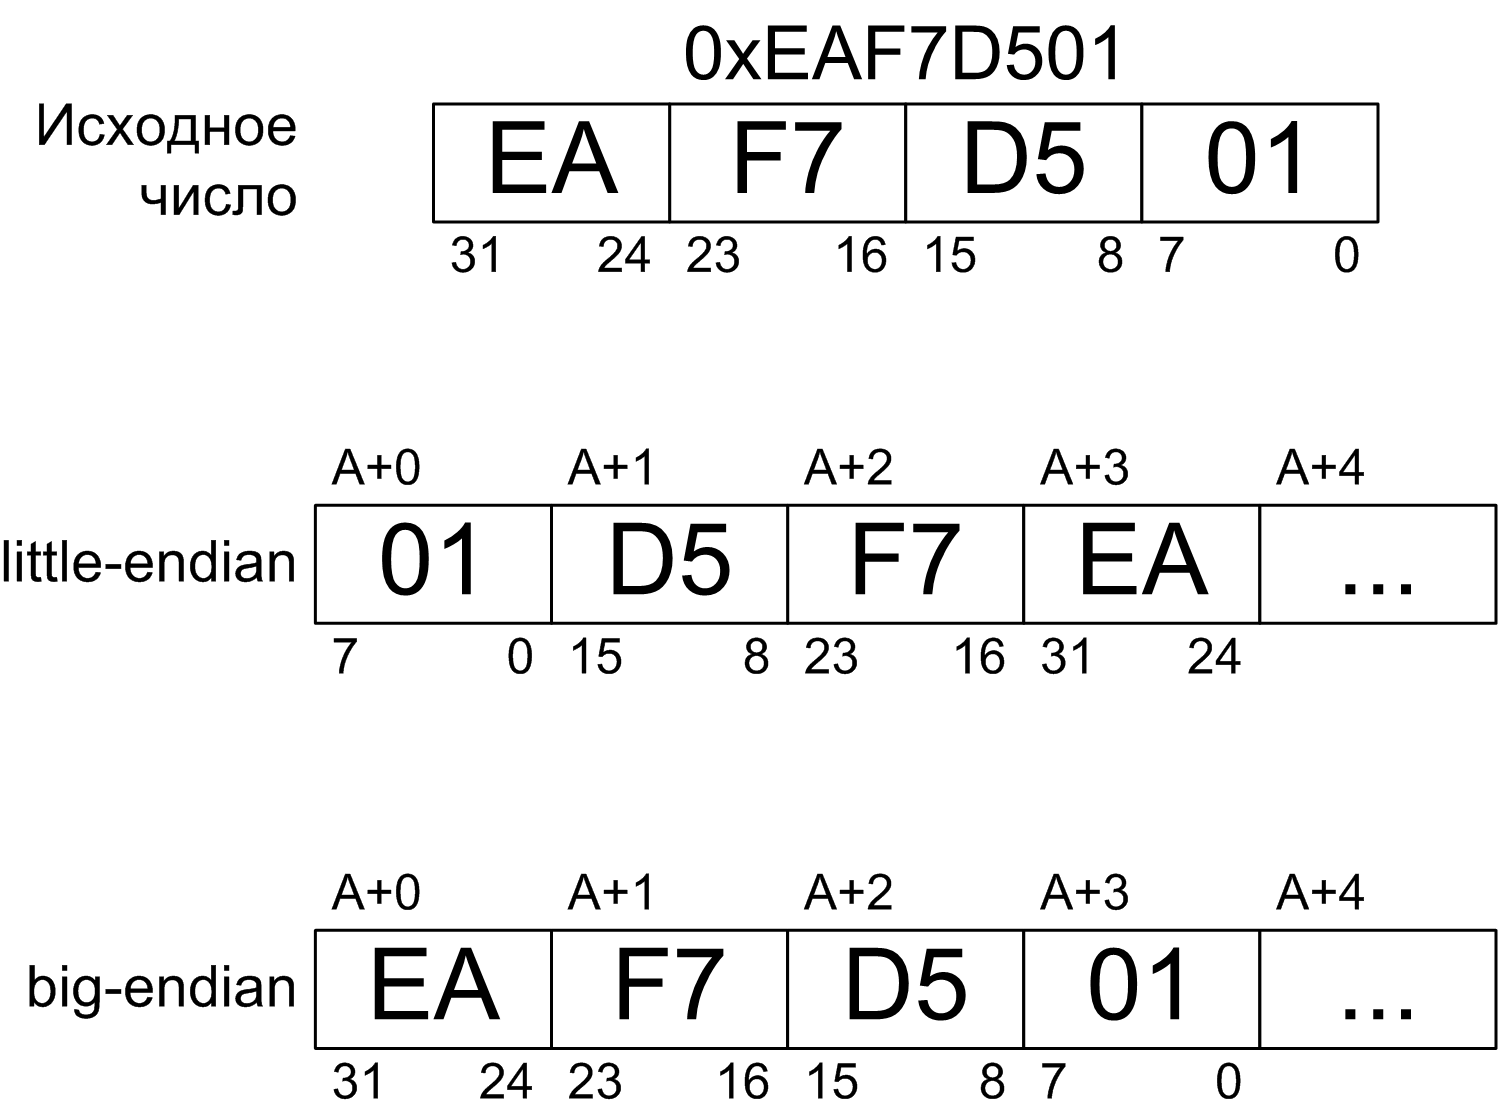
\includegraphics[width=0.65\textwidth]{fig/byteOrder}
    \end{center}
\end{frame}


\subsection{Прямой код}

\begin{frame}
    \frametitle{Прямой код}
    \framesubtitle{Построение прямого кода числа $x$}

    Старший разряд прямого кода называют <<знаковым>>. Знаковый разряд содержит 0, если $x\ge 0$, и 1, если $x<0$. Т.е. знак <<+>> кодируется нулем, а <<->> --- единицей:
    \[
        Sign(x)=
        \begin{cases}
            0, & \text{если $x \ge 0$},\\
            1, & \text{если $x < 0$}.
        \end{cases}
    \]
    
    Остальные разряды содержат двоичное представление $|x|$:
    \[
        \SignedAny{n-1}{}{$Sign(x)$}{Двоичное представление $|x|$}
    \]
\end{frame}

\begin{frame}
    \frametitle{Прямой код}
    \framesubtitle{Примеры кодирования в 4-х разрядной сетке}

    \begin{itemize}
        \item \SignedNibble{0}{011} $\Leftrightarrow$ $3$;
        \item \SignedNibble{1}{101} $\Leftrightarrow$ $-5$;
        \item \SignedNibble{0}{000} $\Leftrightarrow$ $0$;
        \item \SignedNibble{1}{000} $\Leftrightarrow$ запрещенный здравым смыслом ${-0}$;
    \end{itemize}
\end{frame}

\begin{frame}
    \frametitle{Прямой код}
    \framesubtitle{Особенности}

    \begin{itemize}
        \item Любим студентами <<за простоту>>.
        \item Имеется запрещенная комбинация. Знаковый разряд 1, а представление модуля содержит нули:
        \[
            \SignedAny{n-1}{}{1}{0$\cdots$0}
        \]
        \item Арифметическое сложение прямых кодов не имеет смысла.
        \item В $n$-разрядной сетке можно представить целые числа:
        \begin{itemize}
            \item Минимальное: $-(2^{n-1} - 1)$;
            \item Максимальное: $(2^{n-1} - 1)$.
        \end{itemize}
    \end{itemize}
\end{frame}


\subsection{Дополнительный код}

\begin{frame}
    \frametitle{Дополнительный код}
    \framesubtitle{Построение дополнительного кода числа $x$}

    Дополнительный код числа $x$ будем обозначать $\DC{x}$ и находить как
    \[
        \DC{x}=
        \begin{cases}
            \overline{|x|}+1, &\text{если $x<0$},\\
            |x|,              &\text{если $x\ge 0$},
        \end{cases}
    \]
    где $\overline{|x|}$ --- инверсия бит в двоичном представлении модуля числа $x$.
    
    \begin{block}{}
        При таком подходе\footnote{Если количества разрядов сетки достаточно для представления} старший разряд кода можно считать знаковым: он как и в прямом коде будет содержать 0, если число положительно и 1 в противном случае.
    \end{block}
\end{frame}

\begin{frame}
    \frametitle{Дополнительный код}
    \framesubtitle{Примеры кодирования в 4-х разрядной сетке}

    \begin{itemize}
        \item $3$ $\Rightarrow$ \SignedNibble{0}{011}
        \item $-5$ $\Rightarrow$ \SignedNibble{1}{011}
        \item $-6$ $\Rightarrow$ \SignedNibble{1}{010}
        \item $-8$ $\Rightarrow$ \SignedNibble{1}{000}
        \item \fbox{$-9 \not\Leftrightarrow \SignedNibble{0}{111}$} --- за пределами предствления в 4-х разрядах
    \end{itemize}
\end{frame}

\begin{frame}
    \frametitle{Дополнительный код}
    \framesubtitle{Декодирование числа из $n$-разрядного кода $\DC{x}$}

    Если старший разряд кода --- единица, то знак числа отрицательный, в противном случае --- положительный.
    
    Двоичное представление модуля числа извлекается по схожим правилам:
    \[
        |x|=
        \begin{cases}
            \overline{\DC{x}}+1, &\text{если в знаковом разряде кода 1}, \\
            \DC{x},              &\text{если в знаковом разряде кода 0}.
        \end{cases}
    \]
\end{frame}

\begin{frame}
    \frametitle{Дополнительный код}
    \framesubtitle{Примеры декодирования в 4-х разрядной сетке}

    \begin{itemize}
        \item \SignedNibble{0}{010} $\Rightarrow$ $2$
        \item \SignedNibble{1}{101} $\Rightarrow$ $-3$
        \item \SignedNibble{1}{110} $\Rightarrow$ $-2$
        \item \SignedNibble{0}{111} $\Rightarrow$ $7$
        \item \SignedNibble{1}{111} $\Rightarrow$ $-1$
    \end{itemize}
\end{frame}

\begin{frame}
    \frametitle{Дополнительный код}
    \framesubtitle{Характерные дополнительные коды чисел в $n$-разрядной сетке}

    \begin{itemize}
        \item $\DC{-1}=\underbrace{11\cdots 11}_n$
        \item $\DC{-2^{n-1}}=\underbrace{10\cdots 00}_n$
        \item $\DC{2^{n-1}-1}=\underbrace{01\cdots 11}_n$
        \item $\DC{-2}=\underbrace{11\cdots 10}_n$
        \item $\DC{0}=\underbrace{00\cdots 00}_n$
        \item $\DC{1}=\underbrace{00\cdots 01}_n$
    \end{itemize}
\end{frame}

\begin{frame}
    \frametitle{Дополнительный код}
    \framesubtitle{Особенности}

    \begin{itemize}
        \item Запрещенных комбинаций нет.
        \item На практике в целочисленной арифметике используется в 100\% случаев.
        \item Арифметическое сложение дополнительных кодов дает дополнетельный код результата или переполнение разрядной сетки.
        \item В $n$-разрядной сетке можно представить целые числа:
        \begin{itemize}
            \item Минимальное: $-2^{n-1}$;
            \item Максимальное: $(2^{n-1}-1)$.
        \end{itemize}
    \end{itemize}
\end{frame}

\begin{frame}
    \frametitle{Дополнительный код}
    \framesubtitle{Сложение дополнительных кодов}

    В результате сложения дополнительных кодов операндов, получается дополнительный код результата или разрядная сетка переполняется. Признаком переполнения может служить следующий признак:
    \begin{block}{}
        если складывались дополнительные коды операндов одного знака, а получился результат противоположного знака --- призошло ПРС\footnote{Переполнение Разрядной Сетки}
    \end{block}
\end{frame}

\begin{frame}
    \frametitle{Дополнительный код}
    \framesubtitle{Примеры сложения в 4-х разрядной сетке}
    
    Корректные результаты:
    \begin{columns}
        \column{.20\textwidth}
            \begin{block}{$2+3=5$}
                 \center
                 \Addition{0010}
                          {0011}
                          {0101}
            \end{block}
        \column{.20\textwidth}
            \begin{block}{${-5}-3=-8$}
                 \center
                 \Addition{1011}
                          {1101}
                          {1000}
            \end{block}
        \column{.20\textwidth}
            \begin{block}{${-1}+6=5$}
                 \center
                 \Addition{1111}
                          {0110}
                          {0101}
            \end{block}
        \column{.20\textwidth}
            \begin{block}{$3-6={-3}$}
                 \center
                 \Addition{0011}
                          {1010}
                          {1101}
            \end{block}
    \end{columns}

    ПРС:
    \begin{columns}
        \column{.20\textwidth}
            \begin{block}{$5+7\neq -4$}
                 \center
                 \Addition{0101}
                          {0111}
                          {1100}
            \end{block}
        \column{.20\textwidth}
            \begin{block}{$5+3\neq -8$}
                 \center
                 \Addition{0101}
                          {0011}
                          {1000}
            \end{block}
        \column{.20\textwidth}
            \begin{block}{$-3-7\neq 6$}
                 \center
                 \Addition{1101}
                          {1001}
                          {0110}
            \end{block}
        \column{.20\textwidth}
            \begin{block}{$-8-1\neq 7$}
                 \center
                 \Addition{1000}
                          {1111}
                          {0111}
            \end{block}
    \end{columns}
\end{frame}

\begin{frame}
    \frametitle{Дополнительный код}
    \framesubtitle{Модифицированный дополнительный код}
    
    Видно, что для того, чтобы устранить ПРС, к исходной $n$-разрядной сетке достаточно добавить слева один разряд. При этом диапазон представления исходных операндов остается прежним:$[-2^{n-1},(2^{n-1} - 1)]$. 
    
    \begin{block}{}
        В \emph{модифицированных} кодах под знаковый разряд выделяется два разряда.
    \end{block}

    И если у результата в знаковых разрядах получилась комбинация, отличная от \Number{00} или \Number{11}, то произошло ПРС\footnote{Хотя в $(n+1)$-разрядной сетке (в немодифицированном $(n+1)$-разрядном коде) результат корректен}.
    
    \begin{block}{}
        О ПРС теперь можно судить, не зная знаки исходных операндов.
    \end{block}
\end{frame}

\begin{frame}
    \frametitle{Модифицированный дополнительный код}
    \framesubtitle{Примеры сложения в модифицированной 4-х разрядной сетке}
    
    Корректные результаты (комбинации знаков \Number{00},\Number{11}):
    \begin{columns}
        \column{.20\textwidth}
            \begin{block}{$2+3=5$}
                 \center
                 \Addition{00010}
                          {00011}
                          {00101}
            \end{block}
        \column{.20\textwidth}
            \begin{block}{${-5}-3=-8$}
                 \center
                 \Addition{11011}
                          {11101}
                          {11000}
            \end{block}
        \column{.20\textwidth}
            \begin{block}{${-1}+6=5$}
                 \center
                 \Addition{11111}
                          {00110}
                          {00101}
            \end{block}
        \column{.20\textwidth}
            \begin{block}{$3-6={-3}$}
                 \center
                 \Addition{00011}
                          {11010}
                          {11101}
            \end{block}
    \end{columns}

    ПРС (комбинации знаков \Number{01},\Number{10}):
    
    \begin{columns}
        \column{.20\textwidth}
            \begin{block}{$5+7\not\equiv 12$}
                 \center
                 \Addition{00101}
                          {00111}
                          {01100}
            \end{block}
        \column{.20\textwidth}
            \begin{block}{$5+3\not\equiv  8$}
                 \center
                 \Addition{00101}
                          {00011}
                          {01000}
            \end{block}
        \column{.20\textwidth}
            \begin{block}{$-3-7\not\equiv -10$}
                 \center
                 \Addition{11101}
                          {11001}
                          {10110}
            \end{block}
        \column{.20\textwidth}
            \begin{block}{$-8-1\not\equiv -9$}
                 \center
                 \Addition{11000}
                          {11111}
                          {10111}
            \end{block}
    \end{columns}
\end{frame}

\begin{frame}
    \frametitle{Сдвиг дополнительного кода}
    
    При сдвиге дополнительного кода числа \emph{вправо}, освобождающийся старший разряд ($msb$) должен заполняться своим значением до сдвига (т.к. знак числа не должен меняться). Это не всегда приводит к ожидаемому уменьшению (отрицательного) числа вдвое:
    \begin{tabular}{l|l}
        $shl(10)=\overrightarrow{\Number{001010}}=\Number{000101}=5$
            & $shl(-10)=\overrightarrow{\Number{110110}}=\Number{111011}=-5$ \\
        $shl(9)=\overrightarrow{\Number{001001}}=\Number{000100}=4$
            & $shl(-9)=\overrightarrow{\Number{110111}}=\Number{111011}=-5$ \\
        $shl(1)=\overrightarrow{\Number{000001}}=\Number{00000}=0$
            & $shl(-1)=\overrightarrow{\Number{111111}}=\Number{111111}=-1$ \\
    \end{tabular}
    Если требуется, чтобы при сдвиге кода вправо модуль представляемого числа уменьшался вдвое, то к результату после сдвига нужно прибавить $(lsb\land msb)$ до сдвига.
    
    При сдвиге дополнительного кода \emph{влево} освобождающийся младший разряд заполняется нулём. Это (при отсутствии ПРС) приводит к увеличению числа вдвое.
\end{frame}

\begin{frame}
    \frametitle{Дополнительный код}
    \framesubtitle{Естественность представления отрицательных чисел}
    
    \[
        \begin{array}{ll}
            {-52} = 2\cdot {-26} + 0; & \Rightarrow a_0 = 0; \\
            {-26} = 2\cdot {-13} + 0; & \Rightarrow a_1 = 0; \\
            {-13} = 2\cdot {-7} + 1;  & \Rightarrow a_2 = 1; \\
            {-7}  = 2\cdot {-4} + 1;  & \Rightarrow a_3 = 1; \\
            {-4}  = 2\cdot {-2} + 0;  & \Rightarrow a_4 = 0; \\
            {-2}  = 2\cdot {-1} + 0;  & \Rightarrow a_5 = 0; \\
            {-1}  = 2\cdot {-1} + 1;  & \Rightarrow a_6 = 1; \\
            {-1}  = 2\cdot {-1} + 1;  & \Rightarrow a_7 = 1; \\
            \cdots                    & \cdots \\
        \end{array}
    \]
    $-52=(1\cdots 11001100)_2.$
\end{frame}


\subsection{Обратный код}
            
\begin{frame}
    \frametitle{Обратный код}
    \framesubtitle{Построение обратного кода числа $x$}

    Обратный код числа $x$ будем обозначать $\OC{x}$ и находить как
    \[
        \OC{x}=
        \begin{cases}
            \overline{|x|},   &\text{если $x<0$},\\
            |x|,              &\text{если $x\ge 0$},
        \end{cases}
    \]
    где $\overline{|x|}$ --- инверсия бит в двоичном представлении модуля числа $x$.
    
    \begin{block}{}
        При таком подходе\footnote{Если количества разрядов сетки достаточно для представления} старший разряд кода можно считать знаковым: он как и в прямом коде будет содержать 0, если число положительно и 1 в противном случае.
    \end{block}
\end{frame}

\begin{frame}
    \frametitle{Обратный код}
    \framesubtitle{Декодирование числа из $n$-разрядного кода $\OC{x}$}

    Если старший разряд кода --- единица, то знак числа отрицательный, в противном случае --- положительный.
    
    Модуль числа:
    \[
        |x|=
        \begin{cases}
            \overline{\OC{x}}, &\text{если в знаковом разряде кода 1}, \\
            \OC{x},            &\text{если в знаковом разряде кода 0}.
        \end{cases}
    \]
\end{frame}

\begin{frame}
    \frametitle{Обратный код}
    \framesubtitle{Примеры кодирования-декодирования в 4-х разрядной сетке}

    \begin{itemize}
        \item \SignedNibble{0}{011} $\Leftrightarrow$ $3$;
        \item \SignedNibble{1}{010} $\Leftrightarrow$ $-5$;
        \item \SignedNibble{1}{001} $\Leftrightarrow$ $-6$;
        \item \SignedNibble{0}{000} $\Leftrightarrow$ $0$;
        \item \SignedNibble{1}{000} $\Leftrightarrow$ $-7$;
        \item \SignedNibble{1}{111} --- запрещенный здравым смыслом ${-0}$.
    \end{itemize}
\end{frame}

\begin{frame}
    \frametitle{Обратный код}
    \framesubtitle{Особенности}

    \begin{itemize}
        \item Любим <<за простоту>> получения, ненавидим <<за необходимость коррекции>>.
        \item Запрещенной комбинацией являются единицы во всех разрядах кода.
        \item Арифметическое сложение обратных кодов дает: 
        \begin{itemize}
            \item правильный обратный код результата;
            \item обратный код результата, \emph{требующий коррекции};
            \item переполнение разрядной сетки.
        \end{itemize}
        \item В $n$-разрядной сетке можно представить целые числа:
        \begin{itemize}
            \item Минимальное: $-(2^{n-1} - 1)$;
            \item Максимальное: $(2^{n-1} - 1)$.
        \end{itemize}
    \end{itemize}
\end{frame}

\begin{frame}
    \frametitle{Сложение обратных кодов}

    Алгоритм проверки результата сложения обратных кодов следующий.
    \begin{enumerate}
        \item Если требуется, выполнить коррекцию результата.
        \begin{block}{}
            Признак: единица переноса из старшего разряда.
            
            Коррекция: прибавить 1 к младшему разряду кода результата.
        \end{block}
        \item Если требуется, зафиксировать ПРС и выйти.
        \begin{block}{}
            Признак: складывались обратные коды операндов одного знака, а получился код противоположного знака.
        \end{block}
        \item Если требуется, скорректировать ($-0\mapsto 0$).
        \begin{block}{}
            Коррекция: $(11\cdots 11)_2\mapsto (00\cdots 00)_2$.
        \end{block}
        \item Фиксировать правильный результат.
    \end{enumerate}
\end{frame}

\begin{frame}
    \frametitle{Обратный код}
    \framesubtitle{Примеры сложения в 4-х разрядной сетке}
    
    Корректные результаты:
    \begin{columns}
        \column{.20\textwidth}
            \begin{block}{$2+3=5$}
                 \center
                 \Addition{0010}
                          {0011}
                          {0101}
            \end{block}
        \column{.20\textwidth}
            \begin{block}{${-5}-2=-7$}
                 \center
                 \Addition{1010}
                          {1101}
                          {0111}
                          
                 Коррекция:
                          
                 \Addition{0111}
                          {0001}
                          {1000}
            \end{block}
        \column{.20\textwidth}
            \begin{block}{${-1}+6=5$}
                 \center
                 \Addition{1110}
                          {0110}
                          {0100}

                 Коррекция:
                          
                 \Addition{0100}
                          {0001}
                          {0101}
            \end{block}
        \column{.20\textwidth}
            \begin{block}{$3-6={-3}$}
                 \center
                 \Addition{0011}
                          {1001}
                          {1100}
            \end{block}
    \end{columns}
\end{frame}

\begin{frame}
    \frametitle{Обратный код}
    \framesubtitle{Примеры сложения в 4-х разрядной сетке}
    
    Ноль:
    \begin{columns}
        \column{.3\textwidth}
            \begin{block}{$2-2=0$}
                 \center
                 \Addition{0010}
                          {1101}
                          {1111}
                          
                 Замена $-0\mapsto 0$:
                          
                 \Number{0000}
            \end{block}
    \end{columns}
\end{frame}

\begin{frame}
    \frametitle{Обратный код}
    \framesubtitle{Примеры сложения в 4-х разрядной сетке}
    
    ПРС:
    \begin{columns}
        \column{.20\textwidth}
            \begin{block}{$5+7\neq -3$}
                 \center
                 \Addition{0101}
                          {0111}
                          {1100}
            \end{block}
        \column{.20\textwidth}
            \begin{block}{$5+3\neq -7$}
                 \center
                 \Addition{0101}
                          {0011}
                          {1000}
            \end{block}
        \column{.20\textwidth}
            \begin{block}{$-3-7\neq 5$}
                 \center
                 \Addition{1100}
                          {1000}
                          {0100}
                          
                 Коррекция:
                 
                 \Addition{0100}
                          {0001}
                          {0101}
            \end{block}
        \column{.20\textwidth}
            \begin{block}{$-5-3\neq 7$}
                 \center
                 \Addition{1010}
                          {1100}
                          {0110}
                          
                 Коррекция:
                 
                 \Addition{0110}
                          {0001}
                          {0111}
            \end{block}
    \end{columns}
\end{frame}

\begin{frame}
    \frametitle{Обратный код}
    \framesubtitle{Модифицированный обратный код}
    
    Обоснование модификации такое же, как и в дополнительном коде. Если исходная сетка $n$-разрядная, а модифицированная $(n+1)$-разрядная, то диапазон представления исходных операндов остается прежним:$[-(2^{n-1} - 1),(2^{n-1} - 1)]$. 
    
    \begin{block}{}
        В \emph{модифицированном} коде знак кодируется двумя разрядами.
    \end{block}

    И если у результата в знаковых разрядах получилась комбинация, отличная от \Number{00} или \Number{11}, то произошло ПРС. Алгоритм сложения остается прежним.
    
    \begin{block}{}
        О ПРС можно судить, не зная знаки исходных операндов.
    \end{block}
\end{frame}

\begin{frame}
    \frametitle{Модифицированный обратный код}
    \framesubtitle{Примеры сложения в модифицированной 4-х разрядной сетке}
    
    Корректные результаты:
    \begin{columns}
        \column{.20\textwidth}
            \begin{block}{$2+3=5$}
                 \center
                 \Addition{00010}
                          {00011}
                          {00101}
            \end{block}
        \column{.20\textwidth}
            \begin{block}{${-5}-2=-7$}
                 \center
                 \Addition{11010}
                          {11101}
                          {10111}
                          
                 Коррекция:
                          
                 \Addition{10111}
                          {10001}
                          {11000}
            \end{block}
        \column{.20\textwidth}
            \begin{block}{${-1}+6=5$}
                 \center
                 \Addition{11110}
                          {00110}
                          {00100}

                 Коррекция:
                          
                 \Addition{00100}
                          {00001}
                          {00101}
            \end{block}
        \column{.20\textwidth}
            \begin{block}{$3-6={-3}$}
                 \center
                 \Addition{00011}
                          {11001}
                          {11100}
            \end{block}
    \end{columns}
\end{frame}

\begin{frame}
    \frametitle{Модифицированный обратный код}
    \framesubtitle{Примеры сложения в модифицированной 4-х разрядной сетке}
    
    Ноль:
    \begin{columns}
        \column{.3\textwidth}
            \begin{block}{$2-2=0$}
                 \center
                 \Addition{00010}
                          {11101}
                          {11111}
                          
                 Замена $-0\mapsto 0$:
                          
                 \Number{00000}
            \end{block}
    \end{columns}
\end{frame}

\begin{frame}
    \frametitle{Модифицированный обратный код}
    \framesubtitle{Примеры сложения в модифицированной 4-х разрядной сетке}
    
    ПРС:
    \begin{columns}
        \column{.20\textwidth}
            \begin{block}{$5+7\not\equiv 12$}
                 \center
                 \Addition{00101}
                          {00111}
                          {01100}
            \end{block}
        \column{.20\textwidth}
            \begin{block}{$5+3\not\equiv 8$}
                 \center
                 \Addition{00101}
                          {00011}
                          {01000}
            \end{block}
        \column{.20\textwidth}
            \begin{block}{$-3-7\not\equiv -10$}
                 \center
                 \Addition{11100}
                          {11000}
                          {10100}
                          
                 Коррекция:
                 
                 \Addition{10100}
                          {00001}
                          {10101}
            \end{block}
        \column{.20\textwidth}
            \begin{block}{$-5-3\not\equiv -8$}
                 \center
                 \Addition{11010}
                          {11100}
                          {10110}
                          
                 Коррекция:
                 
                 \Addition{10110}
                          {00001}
                          {10111}
            \end{block}
    \end{columns}
\end{frame}

\begin{frame}
    \frametitle{Сдвиг обратного кода}
    При сдвиге обратного кода числа \emph{вправо}, освобождающийся старший разряд ($msb$) должен заполняться своим значением до сдвига:
    \begin{tabular}{l|l}
        $shl(10)=\overrightarrow{\Number{001010}}=\Number{000101}=5$
            & $shl(-10)=\overrightarrow{\Number{110101}}=\Number{111010}=-5$ \\
        $shl(9)=\overrightarrow{\Number{001001}}=\Number{000100}=4$
            & $shl(-9)=\overrightarrow{\Number{110110}}=\Number{111011}=-4$ \\
        $shl(1)=\overrightarrow{\Number{000001}}=\Number{00000}=0$
            & $shl(-1)=\overrightarrow{\Number{111110}}=\Number{111111}=-0$ \\
    \end{tabular}
    
    При сдвиге обратного кода \emph{влево} освобождающийся младший разряд заполняется знаковым ($msb$) разрядом. Это (при отсутствии ПРС) приводит к увеличению числа вдвое.
    \begin{tabular}{l|l}
        $shr(10)=\overleftarrow{\Number{001010}}=\Number{010100}=20$
            & $shr(-10)=\overleftarrow{\Number{110101}}=\Number{101011}=-20$ \\
        $shr(9)=\overleftarrow{\Number{001001}}=\Number{010010}=18$
            & $shr(-9)=\overleftarrow{\Number{110110}}=\Number{101101}=-18$ \\
        $shr(1)=\overleftarrow{\Number{000001}}=\Number{000010}=2$
            & $shr(-1)=\overleftarrow{\Number{111110}}=\Number{111101}=-2$ \\
    \end{tabular}
    
\end{frame}

\begin{frame}
    \frametitle{Обратный и дополнительный коды в любой СС}
    \framesubtitle{Основание: $k$. Цифра: $x_i$. Дополнение $\overline{x_i}=(k - x_i - 1)$}
    
    Например, дополнительный код в десятичной СС (4 разряда):
    \begin{columns}
        \column{.30\textwidth}
            \begin{block}{$731-485=246$}
                 \center
                 \Addition{0731}
                          {9515}
                          {0246}
            \end{block}
        \column{.30\textwidth}
            \begin{block}{$204-690=-486$}
                 \center
                 \Addition{0204}
                          {9310}
                          {9514}
            \end{block}
        \column{.30\textwidth}
            \begin{block}{$100-1000=-900$}
                 \center
                 \Addition{0100}
                          {9000}
                          {9100}
            \end{block}
    \end{columns}
\end{frame}


\section{Фиксированная точка}


\begin{frame}
    \frametitle{Фиксированная точка}

    Для представления вещественного числа $x$:
    \begin{itemize}
        \item В $n$-разрядном формате с фиксированной точкой, разделитель целой и дробной части \emph{мысленно} <<фиксируется>> между $k$ и $(k-1)$ разрядами разрядной сетки.
        
        \[\underbrace{\Number{xxxx}\cdots\Number{xxxx}}_{(n-k)}\Number{,}\underbrace{\Number{xx}\cdots\Number{xx}}_{k}\]
        
        \item В старших $(n-k)$ разрядах сохраняется целая часть $x$, а в младщих $k$ разрядах --- дробная.
    \end{itemize}
\end{frame}


\subsection{Масштабирование}

\begin{frame}
    \frametitle{Фиксированная точка}
    \framesubtitle{Масштабирование}
    
    \begin{itemize}
        \item Для \emph{удобства рассуждений}, договариваются о масштабирующем множителе $M=2^m$ --- \emph{масштабе}. $m\in\mathbb{Z}$.
        
        \item Масштаб одинаков для всех чисел и не меняется.
        
        \item Исходное число $x$ представляется в разрядной сетке некоторым кодом числа $y$. Исходное $x$ из $y$ получается по формуле:
        \[
            x = y\cdot M.
        \]

        \item Компьютер, выполняя операции над представлениями $y$, о существовании масшатба <<не догадывается>>.
        
        \item Выделяют два типа масштабирования:
        
        \begin{itemize}
            \item дробное (мы будем использовать в лекциях для выкладок);
            \item целое (как правило, используется программистами).
        \end{itemize}
    \end{itemize}
\end{frame}

\begin{frame}
    \frametitle{Масштабирование}
    \framesubtitle{Дробное}
    
    \[x=y\cdot M\]
    
    При дробном масштабировании представление числа $x$, т.е. 
    \begin{block}{}
        $y$ --- дробное число с нулевой целой частью.
    \end{block}
    
    Рарзядная сетка хранит разряды дробной части $y$.
    \[
        \raisebox{1.\height}{0.}
        \raisebox{1.\height}{
            \UnsignedAny{n-1}{yyyyy$\cdots$yyyyy}
        }
    \]
    
    Чтобы зафиксировать запятую между $k$ и $(k-1)$ разрядами, выбирается масштаб
    \[
        M=2^{(n-k)}.
    \]
\end{frame}

\begin{frame}
    \frametitle{Масштабирование}
    \framesubtitle{Целое}
    
    \[x=y\cdot M\]
    
    При целом масштабировании представление числа $x$, т.е. 
    \begin{block}{}
        $y$ --- целое число.
    \end{block}
    
    Рарзядная сетка хранит разряды целой части $y$.
    
    \[
        \raisebox{1.\height}{
            \UnsignedAny{n-1}{yyyyy$\cdots$yyyyy}
        }
        \raisebox{1.\height}{.0}
    \]
    
    Чтобы зафиксировать запятую между $k$ и $(k-1)$ разрядами, выбирается масштаб
    \[
        M=2^{-k}.
    \]
\end{frame}

\begin{frame}
    \frametitle{Масштабирование}
    \framesubtitle{Пример}

    Дано число 
    \[
        x=(10111.1011)_2.
    \]
    
    \begin{itemize}
        \item При дробном масштабировании в $\DC{y}$ с масштабом $M=2^{10}$ в 16-разрядной сетке ($y=(0.00000101111011)_2$):
        \[
            \UnsignedTwoBytes{0000010111101100}
        \]
        
        \item При целом масштабировании в $\DC{y}$ с масштабом $M=2^{-5}$ в 16-разрядной сетке ($y=(1011110110.0)_2$):
        \[
            \UnsignedTwoBytes{0000001011110110}
        \]
    \end{itemize}
\end{frame}

\begin{frame}
    \frametitle{Масштабирование}
    \framesubtitle{Пример}

    Дано число 
    \[
        x=-(10111.1011)_2.
    \]
    
    \begin{itemize}
        \item При дробном масштабировании в $\DC{y}$ с масштабом $M=2^7$ в 16-разрядной сетке ($y=-(0.00101111011)_2$):
        \[
            \UnsignedTwoBytes{1101000010100000}
        \]
        
        \item При целом масштабировании в $\DC{y}$ с масштабом $M=2^{-6}$ в 16-разрядной сетке ($y=-(10111101100.0)_2$):
        \[
            \UnsignedTwoBytes{1111101000010100}
        \]
    \end{itemize}
\end{frame}


\subsection{Форматы на практике}

\begin{frame}
    \frametitle{Фиксированная точка}
    \framesubtitle{Форматы, используемые на практике}

    На практике, на уровне команд процессора, форматы с фиксированной запятой используют:
    \begin{itemize}
        \item целочисленное масштабирование;
        \item дополнительный код для представления $y$;
        \item разрядности 1, 2, 4, 8 байт.
    \end{itemize}
\end{frame}


\subsection{Оценка погрешности}

\begin{frame}
    \frametitle{Фиксированная точка}
    \framesubtitle{Оценка погрешности}

    Используем целое масштабирование для представления числа $x$ в $n$-разрядной сетке.
    \begin{itemize}
        \item Абсолютная погрешность $\Delta$ --- половина цены деления. Цена деления $y$ --- 1. Цена деления $x=1\cdot M=2^{-k}$.
        \[
            \Delta=\frac{M}{2}=2^{-(k+1)}.
        \]
        
        \item Для относительной погрешности $\delta=\frac{\Delta}{|x|}$ оценим диапазон.
        \begin{align*}
            &\delta_{max}=\frac{\Delta}{|x|_{min}}=\frac{2^{-(k+1)}}{1\cdot M}=\frac{2^{-(k+1)}}{2^{-k}}=\frac{1}{2} \\
            &\delta_{min}=\frac{\Delta}{|x|_{max}}=\frac{2^{-(k+1)}}{2^{n-1}\cdot M}=\frac{2^{-(k+1)}}{2^{n-1}\cdot 2^{-k}}=\frac{1}{2^n} 
        \end{align*}
    \end{itemize}
\end{frame}

\begin{frame}
    \frametitle{Фиксированная точка}
    \framesubtitle{Оценка погрешности --- выводы}

    \begin{itemize}
        \item Абсолютная погрешность --- константа $\Delta=2^{-(k+1)}$.
        
        \item Относительная погрешность $\delta$ изменяется от чудовищной $50\%$ до ничтожной $\frac{100}{2^n}\%$.
    \end{itemize}
\end{frame}


\section{Плавающая точка}


\begin{frame}
    \frametitle{Плавающая точка}

    В форматах с плавающей точкой, в системе счисления с основанием $k$, вещественное число $x$ представляется следующим образом:
    
    \[x = \FloatExpression{x}{k},\]
    где 
    \begin{block}{}
        \begin{itemize}
            \item $\MantissOf{x}$ --- \emph{мантисса} числа $x$;
            \item $\OrderOf{x}$ --- \emph{порядок} числа $x$.
        \end{itemize}
    \end{block}
    
    При этом мантисса $\MantissOf{x}$ обязательно нормализуется. 
\end{frame}

\begin{frame}
    \frametitle{Плавающая точка}
    \framesubtitle{Правила нормализации}

    \[x = \FloatExpression{x}{k}\]
    
    Умножение на $k^{\OrderOf{x}}$ приводит к переносу точки в $\MantissOf{x}$
    \begin{itemize}
        \item влево, если $\OrderOf{x} < 0$;
        \item вправо, если $\OrderOf{x} > 0$.
    \end{itemize}
    
    Порядок числа $\OrderOf{x}$ подбирается так, чтобы мантисса была \emph{нормализованной}.
    
    \begin{block}{}
        Нормализованная мантисса $\MantissOf{x}$ представляет собой дробное число, старший ($-1$-й) разряд которого содержит ненулевую цифру.
    \end{block}
\end{frame}

    
\subsection{Порядок и характеристика}

\begin{frame}
    \frametitle{Плавающая точка}
    \framesubtitle{Порядок. Описание формата для примера}
    
    \[
        \FloatMyHex{X}{XXXXXXXXX}{X}{XXXXX}
    \]
    
    Мантисса и порядок представляются в прямом коде. Модуль мантиссы представлен в рязрядах $[14:6]$, знак мантиссы в 15-м разряде. Модуль порядка представлен в разрядах $[4:0]$, знак порядка в $5$-м разряде.
\end{frame}

\begin{frame}
    \frametitle{Плавающая точка}
    \framesubtitle{Порядок. Пример}
    
    Представить число $-78.4453125$.
    
    \[-78.4453125 = (-1001110.0111001)_2.\]
    
    Нормализованное представление:
    \[-78.4453125 = (-0.10011100111001)_2\cdot 2^{(+111)_2}.\]

   Результат:
    \[
        \FloatMyHex{1}{100111001}{0}{00111}
    \]
\end{frame}

\begin{frame}
    \frametitle{Плавающая точка}
    \framesubtitle{Порядок. Пример}
    
    Представить число $0.00537109375$.
    
    \[0.00537109375 = (0.00000001011)_2.\]
    
    Нормализованное представление:
    \[0.00537109375 = (0.1011)_2\cdot 2^{(-111)_2}.\]

   Результат:
    \[
        \FloatMyHex{0}{101100000}{1}{00111}
    \]
\end{frame}

\begin{frame}
    \frametitle{Плавающая точка}
    \framesubtitle{Характеристика}
    
    В машинных форматах, применяемых на практике, вместо порядка используют \emph{смещённый} порядок --- \emph{характеристику}. В отличие от порядка, 
    \begin{block}{}
        характеристика --- всегда положительное число. 
    \end{block}
    
    Чтобы получить характеристику $\CharOf{x}$ числа $x$, нужно к его порядку прибавить фиксированную константу $\Delta$ --- смещение:
    \[
        \CharOf{x} = \OrderOf{x} + \Delta.
    \]
    
    Тогда число, представленное в формате, будет определяться следующим образом: 
    \[
        x = m_x\cdot k^{(c_x - \Delta)}.
    \]
\end{frame}
  
\begin{frame}
    \frametitle{Плавающая точка}
    \framesubtitle{Характеристика}
    
    Смещение $\Delta$ выбирается исходя из количества разрядов, отведенных под представлние порядка (а также и характеристики). Допустим, что под представление порядка отведено $n$ двоичных разрядов. 
    
    Если использовать дополнительный код, то диапазон представления порядков будет следующим: 
    \[
        [-2^{n-1},(2^{n-1}-1)].
    \]
    
    Таким образом, смещение $\Delta$ для получения характеристики выбирается так, чтобы при сложении с наименьшим отрицательным числом диапазона представления порядка получался ноль.
    
    Для дополнительного кода: $\Delta = 2^{n-1}$.
\end{frame}
  
\begin{frame}
    \frametitle{Плавающая точка}
    \framesubtitle{Характеристика}

    Использование характеристики вместо порядка дает на практике несколько преимуществ, одно из которых заключается в том, что положительные числа (характеристики) гораздо проще сравнивать друг с другом.
\end{frame}
  
\begin{frame}
    \frametitle{Плавающая точка}
    \framesubtitle{Характеристика. Описание формата для примера}
    
    \[
        \FloatMyCharHex{X}{XXXXXXXXX}{XXXXXX}
    \]
    
    Мантисса представляется в прямом коде. Модуль мантиссы представлен в разрядах $[14:6]$, знак мантиссы в $15$-м разряде. Характеристика представлена в разрядах $[5:0]$, смещение порядка $\Delta=2^5$.
\end{frame}

\begin{frame}
    \frametitle{Плавающая точка}
    \framesubtitle{Характеристика. Пример}
    
    Представить число $-78.4453125$.
    
    \[-78.4453125 = (-1001110.0111001)_2.\]
    
    Нормализованное представление:
    \[-78.4453125 = (-0.10011100111001)_2\cdot 2^{(+111)_2}.\]

   Результат:
    \[
        \FloatMyCharHex{1}{100111001}{100111}
    \]
\end{frame}

\begin{frame}
    \frametitle{Плавающая точка}
    \framesubtitle{Характеристика. Пример}
    
    Представить число $0.00537109375$.
    
    \[0.00537109375 = (0.00000001011)_2.\]
    
    Нормализованное представление:
    \[0.00537109375 = (0.1011)_2\cdot 2^{(-111)_2}.\]

   Результат:
    \[
        \FloatMyCharHex{0}{101100000}{011001}
    \]
\end{frame}

  
\subsection{Форматы на практике}

\begin{frame}
    \frametitle{Плавающая точка}
    \framesubtitle{Форматы, применяемые на практике: ЕС ЭВМ}
    
    ЕС ЭВМ. Используется три варианта формата: короткий (32 бита), длинный (64 бита), расширенный (128 бит). Во всех вариантах используются смешенные порядки (характеристики), занимающие 7 бит (смещение $\Delta = 64$). Старший бит формата содержит знак числа, затем следуют 7 бит характеристики, а оставшиеся разряды занимает модуль мантиссы. Мантисса изображается в 16-ичной системе счисления, т.е. каждые 4 бита мантиссы воспринимаются ЭВМ как шестнадцатеричная цифра. Т.е. 
    \[x=m_x\cdot 16^{(c_x-\Delta)}.\] 
    Мантисса нормализуется так, что после точки (запятой) следует ненулевая шестнадцатеричная цифра, а её целая часть равна нолю.
\end{frame}

\begin{frame}
    \frametitle{Плавающая точка}
    \framesubtitle{Форматы, применяемые на практике: ЕС ЭВМ}

    \[-78.4453125 = (-1001110.0111001)_2.\]

    \[
        \FloatESShort{1}{1000010}{0100 1110 0111 0010 0000 0000}
    \]
    
    \[0.00537109375 = (0.00000001011)_2.\]
    \[
        \FloatESShort{0}{0111111}{0001 0110 0000 0000 0000 0000}
    \]
\end{frame}

\begin{frame}
    \frametitle{Плавающая точка}
    \framesubtitle{Форматы, применяемые на практике: СМ ЭВМ (ПЭВМ)}
    
    СМ ЭВМ. Используется два варианта формата: короткий (32 бита) и длинный (64 бита). Характеристика в обоих вариантах занимает 8 бит ($\Delta = 128$). Старший разряд отводится под знак числа, далее следуют 8 бит характеристики, а остальные разряды занимает модуль мантиссы. Характеристика отражает положение точки в двоичном представлении числа:
    \[x=m_x\cdot 2^{(c_x-\Delta)}.\]
\end{frame}

\begin{frame}
    \frametitle{Плавающая точка}
    \framesubtitle{Форматы, применяемые на практике:  СМ ЭВМ (ПЭВМ)}

    \[-78.4453125 = (-1001110.0111001)_2.\]

    \[
        \FloatPCShort{1}{10000111}{10011100111001000000000}
    \]
    
    \[0.00537109375 = (0.00000001011)_2.\]
    \[
        \FloatPCShort{0}{01111001}{10110000000000000000000}
    \]
\end{frame}

\subsection{Оценка погрешности формата}

\begin{frame}
    \frametitle{Плавающая точка}
    \framesubtitle{Оценка погрешности}

    \[
        x = \FloatExpression{x}{2}
    \]
    
    \begin{itemize}
        \item Абсолютная погрешность зависит от порядка числа:
        \[
            \Delta=
                \frac{2^{-\lVert\MantissOf{x}\rVert}}{2}\cdot 2^{\OrderOf{x}}=
                \frac{2^{(\OrderOf{x} - \lVert\MantissOf{x}\rVert)}}
                     {2}.
        \]
        
        \item Для относительной погрешности $\delta=\frac{\Delta}{|x|}$ оценим диапазон, который, как видно, от порядка числа не зависит.
        \begin{align*}
            &\delta_{max}=\frac{\Delta}{2^{-1}\cdot 2^{\OrderOf{x}}}=
                2^{-\lVert\MantissOf{x}\rVert}
            \\            
            &\delta_{min}=
                \frac{\Delta}
                     {(1-2^{-\lVert\MantissOf{x}\rVert})\cdot 2^{\OrderOf{x}}}= 
                \frac{2^{- \lVert\MantissOf{x}\rVert}}
                     {2\cdot(1-2^{-\lVert\MantissOf{x}\rVert})}\approx 
                     \frac{2^{-\lVert\MantissOf{x}\rVert}}{2}
        \end{align*}
    \end{itemize}
\end{frame}

\begin{frame}
    \frametitle{Плавающая точка}
    \framesubtitle{Оценка погрешности --- выводы}

    \begin{itemize}
        \item Абсолютная погрешность зависит от порядка: чем он больше, тем больше и погрешность представления чисел. 
        \[
            \Delta = \frac{2^{(\OrderOf{x} - \lVert\MantissOf{x}\rVert)}}
                     {2}
        \]        
        
        \item Относительная погрешность $\delta$ --- практически константа и равна (в худшем случае) вкладу младшего разряда мантиссы.
        \[
            \delta = 2^{-\lVert\MantissOf{x}\rVert}
        \]        
        
    \end{itemize}
\end{frame}

        
\appendix

\section{Задания на практику}


\subsection{Проходное}

\begin{frame}
    \frametitle{\TaskSimpleNumber}

    Перевести число $115.43$ 
    \[
        \text{10СС}\to\text{8СС}\to\text{2СС}\to\text{16СС}\to\text{10СС}
    \]
    выбрать необходимое количество знаков в дробной части\footnote{
        Исходя из соображений максимально точного приближения, при переводе дробной части следует использовать бесконечное количество знаков после запятой. Исходя же из экономии аппаратных затрат, следует взять необходимый минимум знаков после запятой, дающий не худшую точность представления. Если число представлено в СС с основанием $k_1$ и дробная часть состоит из $n_1$-й цифры, то при переводе в систему счисления с основанием $k_2$ следует взять $n_2$ знаков после запятой
        \[
            n_2 \ge \left\lceil n_1\frac{\ln{k_1}}{\ln{k_2}} \right\rceil.
        \]
    }. Оценить абсолютную и относительную погрешности представления в 2CC.
\end{frame}
        
\begin{frame}
    \frametitle{\TaskSimpleNumber}

    Какое число представлено в дополнительном коде в формате с фиксированной точкой 
    \[
        \UnsignedTwoBytes{1101101000011101}
    \]
    если:
    \begin{enumerate}
        \item использовалась дробная нормализация и масштаб $2^9$;
        \item использовалась целая нормализация и масштаб $2^{-6}$.
    \end{enumerate}
    Дать оценку минимальной абсолютной погрешности в обоих случаях.
\end{frame}
        
\begin{frame}
    \frametitle{\TaskSimpleNumber}

    Какое число представлено в формате с плавающей точкой
    \begin{align*}
        \FloatMySimpleHex{1100100000}{100011}\\
        \FloatMySimpleHex{0110110000}{000111}
    \end{align*}
    если разряды $[15:6]$ --- мантисса в прямом коде (нормализация: 0 в целой части, после точки --- 1), разряды $[5:0]$ --- порядок в прямом коде.
\end{frame}
        
\begin{frame}
    \frametitle{\TaskSimpleNumber}
    
    Какое число представлено в формате с плавающей точкой
    \begin{align*}
        \FloatMySimpleHex{0101100000}{100011}\\
        \FloatMySimpleHex{1101110000}{011110}
    \end{align*}
    если разряды $[15:6]$ --- мантисса в прямом коде (нормализация: 0 в целой части, после точки --- 1), разряды $[5:0]$ --- характеристика.
\end{frame}
        
\begin{frame}
    \frametitle{\TaskSimpleNumber}
    Представить число $-0,01953125$ в коротком формате EC ЭВМ.
\end{frame}
        
\begin{frame}
    \frametitle{\TaskSimpleNumber}
    Представить число $14.07421875$ в коротком формате СМ ЭВМ.
\end{frame}
        
\begin{frame}
    \frametitle{\TaskSimpleNumber}
    
    Сложить числа в 16-разрядной сетке в формате с фиксированной точкой (целое масштабирование, масштаб $2^{-6}$).
    \begin{enumerate}
        \item $21\frac{18}{32}$ и $-37\frac{3}{16}$;
        \item $-17\frac{11}{32}$ и $-43\frac{13}{16}$.
    \end{enumerate}
    Выполнить проверку результата и оценить погрешности.
\end{frame}

\begin{frame}
    \frametitle{\TaskSimpleNumber}
    
    Определим собственный формат с плавающей точкой. Для представления числа используется шестнадцать двоичных разрядов. Мантисса представляется в прямом коде. Модуль мантиссы представлен в рязрядах $[15:6]$, знак мантиссы в 15-м разряде. Характеристика представлена в разрядах $[5:0]$, смещение порядка $\Delta=2^5$.
    \[
        \FloatMyCharHex{X}{XXXXXXXXX}{XXXXXX}
    \]

    Сложить перечисленные ниже пары чисел (изобразив необходимые действия в формате), выполнить проверку результата и оценить погрешности.
    \begin{enumerate}
        \item $125.75$ и $\frac{5}{128}$;
        \item $65$ и $-\frac{6}{128}$;
        \item $125.625$ и $-126.5$.
    \end{enumerate}
\end{frame}


\subsection{Мускулистым}

\begin{frame}[allowframebreaks]
    \begin{enumerate}
        \item Сложите десятичные числа в дополнительном коде, выберите масштаб и разрядную сетку самостоятельно.
        \begin{enumerate}   
            \item $975.48$ и $-729.503$;
            \item $-795.804$ и $279.35$;
            \item $-795.034$ и $-729.13$.
        \end{enumerate}
        \item Сложите десятичные числа $-975.48$ и $-729.53$ в обратном коде, выберите масштаб и разрядную сетку самостоятельно.
        \begin{enumerate}   
            \item $482.07$ и $-195.053$;
            \item $-675.015$ и $511.39$;
            \item $-851.11$ и $-163.509$.
        \end{enumerate}
        \item Как представить ноль в формате с плавающей запятой?
        \item Когда нет необходимости выполнять сложение мантисс числа в формате с плавающей точкой.
    \end{enumerate}
\end{frame}


\subsection{Мегамозг}

\begin{frame}[allowframebreaks]
    \begin{enumerate}
        \item Обоснуйте коррекность декодирования дополнительного кода.
        \item Доказать, что после коррекции результата сложения обратных кодов запрещенная комбинация <<все единицы>> возникнуть не может.
        \item Доказать или опровергнуть, что в результате сложения обратных кодов комбинация <<все нули>> может получиться только вследствие замены комбинации <<все единицы>>.
        \item Чем <<чревато>> не запрещать комбинацию <<все единицы>> в обратном коде. Если считать комбинацию <<все единицы>> еще одним представлением нуля, повлечет ли это проблемы с определением ПРС или коррекцией?
        \item Продумайте правила сложения в троичной симметричной системе счисления, признаки ПРС, модификацию кода?
    \end{enumerate}
\end{frame}


\section{Самообучение}

\begin{frame}
    \frametitle{Советы самоучке}
    
    Рекомендуемые книги, ставшие классикой: \cite{bib:lisikov:automateBase,bib:saveliev:automateTheory}.
\end{frame}

\begin{frame}[allowframebreaks]{Библиография}
    \bibliographystyle{gost780u}
    \bibliography{./../../../bibliobase}
\end{frame}

\end{document}